\documentclass{jsarticle}
\usepackage{multicol}

% sourcecode highlight
\usepackage{color}
\usepackage{listings,jlisting}

%jlisting (sourcecode highlight)
\lstset{
language={C},
backgroundcolor={\color[gray]{.85}},
basicstyle={\small},
identifierstyle={\small},
commentstyle={\small\ttfamily \color[rgb]{0,0.5,0}},
keywordstyle={\small \color[rgb]{0,0,0}},
ndkeywordstyle={\small},
stringstyle={\small\ttfamily \color[rgb]{0,0,1}},
frame={tb},
breaklines=true,
columns=[l]{fullflexible},
numbers=left,
xrightmargin=0zw,
xleftmargin=3zw,
numberstyle={\scriptsize},
stepnumber=1,
numbersep=1zw,
morecomment=[l]{//}
}

%comment out multiple line
\usepackage{comment}

%image
\usepackage[dvipdfmx]{graphicx}
\usepackage{here}


\title{麻雀点数計算プログラム\ 注釈書}
\author{14EC004\ 飯田頌平}

\begin{document}
\maketitle

\begin{multicols}{2}

\section{はじめに}
本稿は吉田さんの麻雀点数計算プログラム\cite{yoshida}
の注釈書にあたる。

このプログラムはカメラで麻雀の手牌を撮影すると
点数を自動で計算するというものであり、
大まかにサーバ、画像認識、点数計算の三つのモジュールに分かれている。

このうち本稿では画像認識の部分について触れる。
画像認識の実装ファイルTemplateMatching.scala
およびユーザ定義関数の実装ファイルpackage.scala
を付録に掲載するので、参考にしながら読むこと。

\section{プログラムの実行方法}

プログラムはgithub上に上げられているが、
それをcloneするだけでは動作しない。
sbtをインストールした上で、opencvを使用できるようにせねばならない。

Ubuntuであれば、sbtは以下のコマンドでインストールできる。
\begin{lstlisting}[caption=sbt,label=sbt]
$ sudo apt-get install sbt
\end{lstlisting}

opencvは各自自力でコンパイルする必要がある。
公式ドキュメントを参考にして、以下のコマンドを実行して.soファイルを生成する。
\begin{lstlisting}[caption=opencv,label=opencv]
$ git clone git://github.com/Itseez/opencv.git
$ cd opencv
$ mkdir build
$ cd build
$ cmake -DBUILD_SHARED_LIBS=OFF
$ make -j8
\end{lstlisting}

.soファイルはopencv/build/libに生成されるはずである。
もし生成されていない場合は、cmakeの出力結果を確認すること。
To\ be\ builtの項目にjavaとない場合は、java-8-oracleの環境変数を設定できていないので、
\begin{lstlisting}[caption=JAVAHOME,label=j]
$ JAVA_HOME=/usr/lib/jvm/java-8-oracle
\end{lstlisting}
を実行すること。

生成された.soファイルを、cloneしてきたmahjongsディレクトリの下の
mahjongs/recogniser/lib
に置けばsbt環境下でopencvを使用することができるようになる。

\section{画像認識のフロー}

画像認識はパターンマッチングによって行われている。
よって、最初に訓練データからテンプレートを生成し、その後テストデータとテンプレートを照合させて結果を求める。
まずはテンプレートの生成手順を示す。
\begin{enumerate}
\item 雀牌を黒と白で二値化する
\item 雀牌の輪郭を判別し、雀牌だけを切り取る
\item 雀牌から牌ひとつあたりの縦幅と横幅を求める
\item 白と判別された誤差(牌の隅)を黒く塗りつぶす
\item 牌の絵柄部分の輪郭情報を得る
\item 輪郭情報と雀牌のグレースケール画像からテンプレートを生成する
\end{enumerate}

詳細な説明については後述するとして、
次に照合の手順を示す。
\begin{enumerate}
\item 手牌の輪郭を判別し、手牌(純手牌+鳴牌)だけを切り取る
\item テンプレートと同じサイズにリサイズする
\item 取得した輪郭の頂点数を求める(四角形なら純手牌である)
\item テンプレートから各牌を回転させたイメージを得る
\item 手牌とテンプレート(及び回転イメージ)をテンプレートマッチングで照合する
\item 照合結果に牌種のシーケンスを与え、結果の最大スコアを取り出す
\item 最大スコアを基に矩形を作成し、手牌を矩形領域で塗りつぶす
\item 5.6.7.の手順を再帰的に繰り返すと、手牌が黒く塗りつぶされてゆく。
		  完全に塗りつぶされたら、再帰を終了する
\item 純手牌を第一要素、鳴牌を第二要素のタプルを作り、関数の結果として返す
\end{enumerate}

こうして手牌を認識することができた。
次章以降ではこれらの流れの詳細について述べる。

\section{テンプレートの生成}

テンプレートの生成にあたって、
まずは元画像を用意する。
以下にその要件を示す。
\begin{itemize}
\item 雀牌を4*9の矩形上に隙間なく並べる。矩形は平行になるようにする
\item 牌の位置は固定である。
		  一萬からはじまるSEQが予め定められている
\item 雀牌と背景以外のものを除外する
\item 撮影時に、各牌が等しい高さと幅を持つよう注意する
\item 二値化からの境界値探索を阻害しないよう背景を選ぶ
\end{itemize}

背景には麻雀マットなどを用いれば良い。
また斜めから撮影された画像からは正しいテンプレートが得られないことに気を付ける。

元画像はプログラムへMat型で渡される。
Mat型はopencv\footnote{https://github.com/bytedeco/javacv}のライブラリが提供する行列の型であり、
opencvではこの型で画像データを扱う。
Mat型の内部構造は行列、画素値、画素のデータ型である。
createTemplateの引数matが元画像のデータを示す変数である。

matに対して最初に行われる処理は、定数MaxResolutionのサイズに近づくよう
resizeで画像サイズを修正する。
大きい画像であると処理時間が増えてしまうため、これによって効率化する。

次に雀牌と背景を識別し、雀牌だけを切り取るcropを実行する。
cropは元画像を引数に取り、Buffer型のシーケンスで識別結果の画像を返す。
(なおBufferはタプルであり、画像だけでなく輪郭の二次元配列も返しているが、
この値はcreateTemplateでは参照しない。)

cropの実装は、
まずfindContoursによって元画像を輪郭で分離し、
minAreaRectで矩形を得て、
warpAffineで矩形の傾きを底面と垂直になるよう修正し、
getRectSubPixで矩形領域のピクセル値を得ることで、
入力画像を輪郭毎に分離した上で補正をかけた画像を得るようになっている。

白と黒で二値化されたテンプレート画像は、
牌の集合の縁は白、背景は黒と別の色で分けられているため、
findCountoursによって輪郭を得られるようになっている。
得た輪郭countourのメソッドtoArrayを用いれば、
minAreaRectで矩形を引くべき座標を得られるのである。

こうして得られた分離後の画像のシーケンス(返り値はBuffer型であることに注意)から
headOptionを使うことで先頭要素を取り出せる。
findContoursでは大きさ順に画像をソートする作用があるので、
先頭要素には一番大きな画像が入る。
一番大きな画像が雀牌であるという前提であるなら、
この先頭要素は雀牌であるため、雀牌のテンプレートは引数templateに束縛される。

thresholdによってテンプレートを黒と白で二値化し、
widthとheightに牌ひとつあたりの幅と高さを代入する。
このとき雀牌の並びが4*9でなかったとき、想定外の値を取ってしまうので注意すること。

こうして得られた二値化後の画像について見てみると、
牌の模様が白、牌の背景が黒で表されていることが分かる。
しかしそれと同時に、牌と牌の間なども白く判定されてしまっている。
牌の模様以外が白と認識されてはパターンマッチに失敗するため、
次はこの誤判定部分を黒く塗りつぶす。
それにはfloodFillを使う。
floodFillは座標を指定し、連結部分を指定した色で塗りつぶす関数である。
これを牌と牌の間にすべてに対して実行することで、
誤判定が塗りつぶされる。
floodFillの補完として、dilateを使用する。
dilateは膨張処理によってノイズを消す効果があり、
ターゲットの周辺に1ピクセルでも白があれば、ターゲットを白に置き換える処理を行う。
これによって牌の模様をはっきりとさせる。

そして牌の模様だけを抽出する。
findContoursによって再び輪郭ごとの分離をかければ、
模様だけを抽出することができる。
四筒のように模様が複数に分離されてしまうケース(二筒ふたつとして認識される)の場合は、
convexHullによって結合する。
convexHullは点群の凸包を得た後に外接する矩形で近似する。
最後に、得られた模様の中で、もっとも面積の大きなものをsizeに代入する。
マッチングを行う際にはこのサイズを基準にするためである。

ここまでで二値化を通して牌の模様の輪郭情報を抽出する処理を行った。
今度はこれをグレースケール画像に適用し、牌一種類ごとのテンプレートを得る。

それにはgridを用いる。
gridはsubmatを実装に含み、元画像から矩形範囲を抽出できる関数である。
gridで牌を4*9に区切り、zipで牌ごとに模様の輪郭の情報を付与し、
それらにflatMapを挟んでgetRectSubPixをかけることによって、
輪郭だけが抽出されたすべての牌のテンプレートを得ることができる。

以上でテンプレートの生成が完了した。

\section{テストデータとの照合}

照合は関数recognizeによって実装されている。
この引数matに手牌の画像データを、templatesにテンプレートの画像データを渡す。

手牌のデータはcropによって背景から切り離される。
しかしテンプレートをcropで切り離したときと違い、
この場合は牌のデータが複数に分かれる。
手牌には純手牌と鳴牌があり、鳴牌は純手牌と離して置くためだ。

手牌のデータはcollectによってhandに束縛される。
handをテンプレートのサイズに合わせてリサイズし、
頂点数を求め純手牌か否かの情報をedgeに代入して、
テンプレートに向きを回転させた牌を加えてtilesに代入すると、
いよいよgoでパターンマッチを行う。
	
goの内部では、まず各テンプレートに対してopencvのテンプレートマッチング関数たるmatchTemplateを呼ぶ。
その結果がresultへと代入されるので、
minMaxLocを通して最高スコアと最低スコアの情報を取り出し、
使用したテンプレートとスコア情報のタプルをlocsに加えてゆく。
この手順をすべてのテンプレートに対して実行する。
minMaxLocの返り値はドキュメントによると\cite{minMaxLoc}
Core.MinMaxLocResult型である。
座標を返すmaxLocフィールドと値を返すmaxValフィールドを参照することで最高スコアの情報を得ることができる。

すべてのテンプレート(及びその回転)に対してのマッチングの結果locsから、
loc値が最大となるものをmaxByによって取得し、変数((tile,loc),i)に代入する。
スコアが最大となる位置はloc.maxLocで参照でき、
それにテンプレートの大きさtile.sizeを組み合わせることで、
マッチした手牌の輪郭rectを得られる。
rectの実装では、最大スコアの場所とサイズから、基準点と縦横のサイズ情報を持つ矩形を作成している。

ここでgoの引数を見てみる。
goの引数はrectsであり、
それはrectと、そのインデックス番号のタプルのシーケンスである。
goは再帰を前提としており、このシーケンスrectsは再帰のたびに認識結果を積み重ねてゆく。

rectangleによってマッチングした牌の輪郭部分に矩形を描き、矩形を領域を塗りつぶすと、
goを再帰する。
このときシーケンスである引数rectsにマッチした牌rectを加えており、
rectsはすべての牌についてのマッチングが終了した時には関数goの返り値となる。

矩形領域がすべて塗りつぶされたあとは、
適当な地点が最大スコアとして返り、そこからそのループでのrectが得られるが、
intersectsによって現在のrectと過去のrect(rectsに保存)の矩形領域が重なっているか否かの判別を行い、
重なっていた場合にマッチング終了という判定を下す。

マッチングを終えたら結果を手牌の位置順にソートし、シーケンス情報だけを取り出しindicesに代入する。
最後に純手牌か否かの判別を改めて行い、その結果とindicesのタプルをresultに代入していく。

resultは純手牌および鳴牌のまとまり毎に要素数がひとつずつ増える構造であり、
最終的に、純手牌と鳴牌のシーケンスのタプルがrecognizeの返り値となる。

\section{matchTemplateについて}

opencvにおけるテンプレートマッチングを行うメソッドmatchTemplateは、以下の引数を取る。
\begin{enumerate}
\item image,\ テンプレートの探索対象となる画像。8ビットまたは32ビットの浮動小数点型
\item templ,\ 探索されるテンプレート。imageと同じデータ型である必要がある
\item result,\ 比較結果のマップ
\item method,\ 比較方法の指定
\end{enumerate}

プログラムではmethodにTM\_CCORR\_NORMEDを指定している。
これは数式で表すと
\begin{figure}[H]
  \begin{center}
    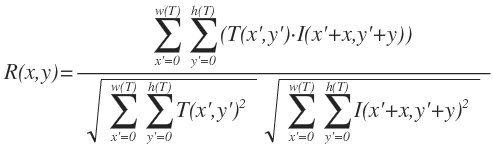
\includegraphics[clip,width=7.0cm]{./img/ccorr.png}
    \caption{相互相関関数}
    \label{fig:ccorr}
  \end{center}
\end{figure}
であり、一般に相互相関関数と呼ばれる式である。

この式の意味するところは、テンプレートと対象画像の内積である。
相互相関関数の式の左辺をcosθに、右辺を内積とゲインの商だと見れば、
まさしくベクトルの内積を示していることがわかる。
相互相関関数の左辺は内積の角度cosθを示しており、
cosθが1に近づけば近づくほど、θは小さく、テンプレートと対象画像の領域が近づいていることを意味する。

各ピクセルに対して内積を求める操作は行われ、その総和を以ってスコアとするので、
スコアが大きければ大きいほど、テンプレートとマッチしているという結果になる。
この点は最小誤差によってマッチングを行うmethodSQDIFFとは逆の意味になっているので、
関数matchTemplateの結果resultには注意が必要である。

matchTemplateの結果であるresultについては、スコアのマップ形式で返される。
マップについて説明する。
そもそもテンプレートマッチングとは、
テンプレート画像と対象画像を重ね合わせて画素の差を比較するという行為を、
各ピクセルに対して行うものである。
つまり重ねあわせが行われる範囲でマッチングの結果が得られるのであって、
それは対象画像のサイズとテンプレート画像のサイズの差の範囲である。
この範囲の行列をマップと呼ぶ。(この呼び名はopencvのドキュメント\cite{matchTemplateC}\cite{matchTemplatePy}に即する)
そしてマップの値にはテンプレートマッチングのスコア(相互相関関数の値)が入るのである。

この理論は実際に画像を用意してmatchTemplateを行い、元画像・テンプレート画像のサイズとマップのサイズを比較すれば裏付けられる。
マップのサイズは縦横ともに元画像とテンプレート画像の差に等しい結果が得られる。
そしてこの結果を画像形式に落とし込んだものが、吉田さんの梗概集の図5に示されたマッチング結果である。
マップの値たる相互相関関数の結果は、0から1の範囲で表されているため、
そのままopencvの出力関数を使うと一面真っ黒な画像(図\ref{fig:res})が得られてしまうが、
255を乗ずることで、opencv標準の0から255までの範囲での画素の表現に対応するようになるため、
吉田さんのマッチング結果のような、縞模様状の結果(図\ref{fig:res2})を得ることができる。

\begin{figure}[H]
  \begin{center}
    
\includegraphics[clip,width=7.0cm]{./img/res.png}
    \caption{相互相関関数出力結果1}
    \label{fig:res}
  \end{center}
\end{figure}

\begin{figure}[H]
  \begin{center}
    
\includegraphics[clip,width=7.0cm]{./img/res2.png}
    \caption{相互相関関数出力結果2}
    \label{fig:res2}
  \end{center}
\end{figure}

%\begin{lstlisting}[caption=,label=]
%
%\end{lstlisting}

\end{multicols}

\newpage

\begin{thebibliography}{9}
\bibitem{yoshida}
	Sanshiro Yoshida.mahjongs.\\
	https://github.com/halcat0x15a/mahjongs
\bibitem{minMaxLoc}
	OpenCV 2.4.2 Java API.Core.MinMaxLocResult.\\
	http://docs.opencv.org/java/2.4.2/index.html?org/opencv/core/Core.html
\bibitem{matchTemplateC}
	物体検出-opencv2.2 documentation. \\
	http://opencv.jp/opencv-2svn/cpp/object\_detection.html
\bibitem{matchTemplatePy}
	Object Detection-opencv2.4.10.\\
	http://docs.opencv.org/2.4/modules/imgproc/doc/object\_detection.html
\end{thebibliography}



\newpage

\section{付録}

\subsection{画像認識}
\begin{lstlisting}[caption=TemplateMatching.scala,label=TemplateMatching]
package mahjongs.recognizer
import org.opencv.core._
import org.opencv.imgproc.Imgproc

object TemplateMatching {

  val MaxResolution: Int = 1024 * 1024

  def createTemplate(mat: Mat): Option[(IndexedSeq[Mat], Size)] = {
    crop(resize(mat, MaxResolution)).headOption.map {
      case (template, _) =>
        val mask = threshold(template.clone, true)
        val width = template.cols / 9
        val height = template.rows / 4
        floodFill(mask, (0 until 4).map(_ * height) :+ (mask.rows - 1), 0 until mask.cols)
        floodFill(mask, 0 until mask.rows, (0 until 9).map(_ * width) :+ (mask.cols - 1))
        Imgproc.dilate(mask, mask, new Mat)
        val rects = for (tiles <- grid(mask, 4, 9)) yield {
          for (tile <- tiles) yield {
            val contours = findContours(tile.clone).flatMap(_.toArray)
            if (contours.length > 0)
              Some(convexHull(contours))
            else
              None
          }
        }
        val size = rects.flatten.flatten.map(_.size).maxBy(_.area)
        val tiles = grid(template, 4, 9).zip(rects).flatMap {
          case (tiles, rects) =>
            tiles.zip(rects).map {
              case (tile, rect) =>
                Imgproc.getRectSubPix(tile, size, rect.fold(center(tile))(center), tile)
                tile
            }
        }.take(34)
        (tiles, new Size(width, height))
    }
  }

  def recognize(mat: Mat, templates: Seq[Mat], width: Int, height: Int): (Seq[Int], Seq[Seq[Int]]) = {
    val result = crop(resize(mat, MaxResolution)).collect {
      case (hand, contour) if hand.size.area > 0 =>
        Imgproc.resize(hand, hand, new Size(hand.size.width * height / hand.size.height, height))
        val edge = approxPoly(new MatOfPoint2f(contour.toArray: _*)).rows
        val tiles = templates ++ templates.map(m => flip(m.t, 0)) ++ templates.map(flip(_, -1)) ++ templates.map(m => flip(m.t, 1))
        def go(rects: List[(Int, Rect)]): List[(Int, Rect)] = {
          val locs = for (tile <- tiles) yield {
            val result = new Mat
            Imgproc.matchTemplate(hand, tile, result, Imgproc.TM_CCORR_NORMED)
            (tile, Core.minMaxLoc(result))
          }
          val ((tile, loc), i) = locs.zipWithIndex.maxBy(_._1._2.maxVal)
          val rect = new Rect(loc.maxLoc, tile.size)
          if (rects.forall(pair => !intersects(rect, pair._2))) {
            Imgproc.rectangle(hand, rect.tl, rect.br, new Scalar(0), -1)
            go((i % 34, rect) :: rects)
          } else {
            rects
          }
        }
        val indices = go(Nil).sortBy(_._2.x).map(_._1)
        (edge == 4 && indices.size != 4, indices)
    }.groupBy(_._1).mapValues(_.map(_._2))
    (result(true)(0), result.get(false).toList.flatten)
  }

}
\end{lstlisting}

\subsection{ユーザ定義関数}
\begin{lstlisting}[caption=package.scala,label=package]
package mahjongs
import scala.collection.JavaConverters._
import scala.collection.mutable.Buffer
import org.opencv.core._
import org.opencv.imgcodecs.Imgcodecs
import org.opencv.imgproc.Imgproc

package object recognizer {

  for {
    ext <- sys.props("os.name").toLowerCase match {
      case name if name.contains("nix") => Some("so")
      case name if name.contains("mac") => Some("dylib")
      case _ => None
    }
  } System.load(getClass.getResource(s"/libopencv_java300.$ext").getPath)

  def findContours(mat: Mat): Buffer[MatOfPoint] = {
    val contours = Buffer.empty[MatOfPoint]
    Imgproc.findContours(mat, contours.asJava, new Mat, Imgproc.RETR_EXTERNAL, Imgproc.CHAIN_APPROX_TC89_KCOS)
    contours.sortBy(Imgproc.contourArea)(Ordering.Double.reverse)
  }

  def floodFill(mat: Mat, rows: Seq[Int], cols: Seq[Int]): Mat = {
    val mask = new Mat
    val color = new Scalar(0)
    for (row <- rows; col <- cols if mat.get(row, col)(0) > 0)
      Imgproc.floodFill(mat, mask, new Point(col, row), color)
    mat
  }

  def grid(mat: Mat, rows: Int, cols: Int): IndexedSeq[IndexedSeq[Mat]] = {
    val height = mat.rows / rows
    val width = mat.cols / cols
    for (row <- 0 until rows) yield {
      val rowRange = new Range(row * height, (row + 1) * height)
      for (col <- 0 until cols) yield
        mat.submat(rowRange, new Range(col * width, (col + 1) * width))
    }
  }

  def approxPoly(contour: MatOfPoint2f, epsilon: Double = 0.01): MatOfPoint2f = {
    val curve = new MatOfPoint2f
    Imgproc.approxPolyDP(contour, curve, Imgproc.arcLength(contour, true) * epsilon, true)
    if (curve.rows % 2 == 0)
      curve
    else
      approxPoly(contour, epsilon + 0.01)
  }

  def threshold(mat: Mat, inv: Boolean): Mat = {
    val (tpe, op) = if (inv) (Imgproc.THRESH_BINARY_INV, Imgproc.MORPH_OPEN) else (Imgproc.THRESH_BINARY, Imgproc.MORPH_CLOSE)
    Imgproc.threshold(mat, mat, 0, 255, tpe | Imgproc.THRESH_OTSU)
    Imgproc.morphologyEx(mat, mat, op, new Mat)
    mat
  }

  def crop(mat: Mat): Buffer[(Mat, MatOfPoint)] = {
    for (contour <- findContours(threshold(mat.clone, false))) yield {
      val patch = new Mat
      val rect = Imgproc.minAreaRect(new MatOfPoint2f(contour.toArray: _*))
      Imgproc.warpAffine(mat, patch, Imgproc.getRotationMatrix2D(rect.center, rect.angle, 1), mat.size)
      Imgproc.getRectSubPix(patch, rect.size, rect.center, patch)
      if (rect.angle <= -45) Core.flip(patch.t, patch, 0)
      (patch, contour)
    }
  }

  def convexHull(contours: Seq[Point]): Rect = {
    val hull = new MatOfInt
    Imgproc.convexHull(new MatOfPoint(contours: _*), hull, false)
    Imgproc.boundingRect(new MatOfPoint(hull.toArray.map(contours): _*))
  }

  def flip(mat: Mat, code: Int): Mat = {
    val m = new Mat
    Core.flip(mat, m, code)
    m
  }

  def resize(mat: Mat, max: Int): Mat = {
    val r = math.sqrt(mat.rows * mat.cols / max.toDouble)
    if (r > 1) Imgproc.resize(mat, mat, new Size(mat.size.width / r, mat.size.height / r))
    mat
  }

  def center(mat: Mat): Point =
    new Point(mat.size.width / 2, mat.size.height / 2)

  def center(rect: Rect): Point =
    new Point(rect.x + rect.width / 2, rect.y + rect.height / 2)

  def toMat(bytes: Array[Byte], gray: Boolean): Mat =
    Imgcodecs.imdecode(new MatOfByte(bytes: _*), if (gray) Imgcodecs.CV_LOAD_IMAGE_GRAYSCALE else Imgcodecs.CV_LOAD_IMAGE_COLOR)

  def fromMat(mat: Mat): Array[Byte] = {
    val buf = new MatOfByte
    Imgcodecs.imencode(".png", mat, buf)
    buf.toArray
  }

  def intersects(a: Rect, b: Rect): Boolean =
    math.max(a.x, b.x) < math.min(a.x + a.width, b.x + b.width) && math.max(a.y, b.y) < math.min(a.y + a.height, b.y + b.height)

  def read(filename: String, gray: Boolean): Mat =
    Imgcodecs.imread(filename, if (gray) Imgcodecs.IMREAD_GRAYSCALE else Imgcodecs.IMREAD_COLOR)

}
\end{lstlisting}

\end{document}